%!TEX TS-program = xelatex
 
% Этот шаблон документа разработан в 2014 году
% Данилом Фёдоровых (danil@fedorovykh.ru) 
% для использования в курсе 
% <<Документы и презентации в \LaTeX>>, записанном НИУ ВШЭ
% для Coursera.org: http://coursera.org/course/latex .
% Исходная версия шаблона --- 
% https://www.writelatex.com/coursera/latex/5.2.2
 
\documentclass[a4paper,12pt]{article}
 
%%% Работа с русским языком
\usepackage[english,russian]{babel}   %% загружает пакет многоязыковой вёрстки
\usepackage{fontspec}      %% подготавливает загрузку шрифтов Open Type, True Type и др.
\defaultfontfeatures{Ligatures={TeX},Renderer=Basic}  %% свойства шрифтов по умолчанию
\setmainfont[Ligatures={TeX,Historic}]{Times New Roman} %% задаёт основной шрифт документа
\setsansfont{Comic Sans MS}                    %% задаёт шрифт без засечек
\setmonofont{Courier New}
\usepackage{indentfirst}
\frenchspacing
 
%%% Дополнительная работа с математикой
\usepackage{amsmath,amsfonts,amssymb,amsthm,mathtools} % AMS
\usepackage{icomma} % "Умная" запятая: $0,2$ --- число, $0, 2$ --- перечисление
 %% Номера формул
\mathtoolsset{showonlyrefs=true} % Показывать номера только у тех формул, на которые есть \eqref{} в тексте.

\author{Батарин Егор}
\title{Вопрос по выбору: Работа 4.7.1 "Двойное лучепреломление"}
\date{\today}
 
\begin{document} % конец преамбулы, начало документа
 
\maketitle

\begin{abstract}
	В данной работе изучается зависимость показателя преломления необыкновенной волны от направления в двоякопреломляющем кристалле.
\end{abstract}

\section{Явление двойного лучепреломления}
Запишем уравнения Максвелла с учетом отсутствия сводобный зарядов и токов: 
\[\begin{gathered}
\operatorname{div}\vec D = 0 \hfill \\
\operatorname{rot}\vec E =  - \frac{1}{c}\frac{{\partial \vec B}}{{\partial t}} \hfill \\
\operatorname{div}\vec B = 0 \hfill \\
\operatorname{rot}\vec H = \frac{1}{c}\frac{{\partial \vec D}}{{\partial t}} \hfill \\ 
\end{gathered} \]
Далее учтем, что $\vec H = \vec B$ и будем рассматривать гармонические волны: 
$$\vec E = {{\vec E}_0}{e^{i\omega t - i\vec k\vec r}},\vec H = {{\vec H}_0}{e^{i\omega t - i\vec k\vec r}}$$
Это приводит к следующим соотношениям эквивалетных операций в уравнениях Максвелла:

$$\frac{\partial }{{\partial t}} \to i\omega, \operatorname{div} \to -i\vec k\cdot,\operatorname{rot} \to -i\vec k\times  $$
\newpage
Теперь можно привести уравнения Максвелла к следующему эквивалетному виду:
\[\begin{gathered}
\vec k \cdot \vec D = 0 \hfill \\
\vec k \cdot \vec H = 0 \hfill \\
\vec k \times \vec E = \frac{\omega }{c}\vec H \hfill \\
\vec k \times \vec H =  - \frac{\omega }{c}\vec D \hfill \\ 
\end{gathered} \]
Это приводит к следующему взаимному расположению векторов, показанных на рисунке ниже:
\begin{figure}[h!]
	\begin{center}
		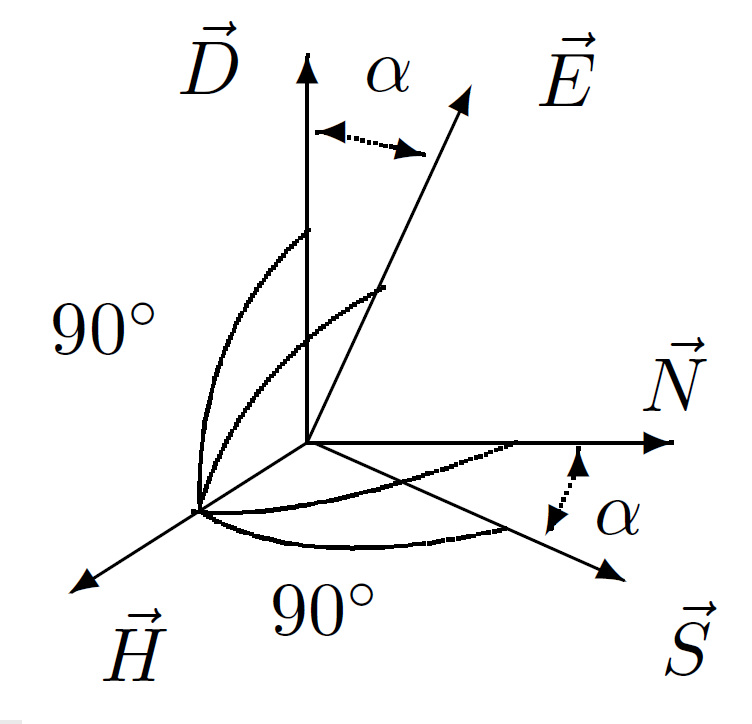
\includegraphics[scale = 0.4]{1.png}
	\end{center}
\end{figure}

Далее рассмотрим явление двойного лучепреломления с точки зрения классической теории дисперсии. Предположим, что направления колебания электроном под действием внешнего гармонического электрического поля $\vec E = \vec E_0 e^{i\omega t}$ ограничены направлением единичного вектора $\vec n$. Тогда уравнение движения электрона можно записать так: 
\[\ddot \vec r + 2\gamma \dot \vec r + \omega _0^2\vec r = \vec n\frac{e}{m}\vec E \cdot \vec n\]
Это приводит к следующему выражению для вектора поляризации: 
\[\vec P = N{{\vec r}_0} = \frac{{N\frac{e}{m}\vec E \cdot \vec n}}{{\omega _0^2 - {\omega ^2} + 2\gamma i\omega }}\vec n = \hat \alpha \vec E\]
В общем случае $\hat \alpha$ представляет с собой матрицу $3\times3$, поскольку направление разрешенных колебаний электрона не обязано совпадать с направлением внешнего электрического поля. Этим определяется тензор диэлектрической проницаемости $\hat \varepsilon = 1 + 4\pi\hat\alpha$. Удачным выбором координатных осей, его можно привести к диагональному виду: $\hat \varepsilon = \operatorname{diag} (\varepsilon_1, \varepsilon_2, \varepsilon_3)$
\newpage
Мы будем рассматривать случай $\varepsilon_1 = \varepsilon_2 = \varepsilon_o, \varepsilon_3 = \varepsilon_e$. В этом случае получаем следущее соотношение между вектором электрического смещения и электрического поля:
\[\vec D = \left( \begin{gathered}
{D_1} \hfill \\
{D_2} \hfill \\
{D_3} \hfill \\ 
\end{gathered}  \right) = \hat \varepsilon \vec E = \left( {\begin{array}{*{20}{c}}
	{{\varepsilon _o}}&0&0 \\ 
	0&{{\varepsilon _o}}&0 \\ 
	0&0&{{\varepsilon _e}} 
	\end{array}} \right)\left( \begin{gathered}
{E_1} \hfill \\
{E_2} \hfill \\
{E_3} \hfill \\ 
\end{gathered}  \right) = \left( \begin{gathered}
{\varepsilon _o}{E_1} \hfill \\
{\varepsilon _o}{E_2} \hfill \\
{\varepsilon _e}{E_3} \hfill \\ 
\end{gathered}  \right)\]
Введем обозначения: 
\[{{\vec D}_ \bot } = \left( \begin{gathered}
{D_1} \hfill \\
{D_2} \hfill \\
0 \hfill \\ 
\end{gathered}  \right) = \left( \begin{gathered}
{\varepsilon _o}{E_1} \hfill \\
{\varepsilon _o}{E_2} \hfill \\
0 \hfill \\ 
\end{gathered}  \right) = {\varepsilon _o}\left( \begin{gathered}
{E_1} \hfill \\
{E_2} \hfill \\
0 \hfill \\ 
\end{gathered}  \right) = {\varepsilon _o}{{\vec E}_ \bot },{{\vec D}_\parallel } = \left( \begin{gathered}
0 \hfill \\
0 \hfill \\
{D_3} \hfill \\ 
\end{gathered}  \right) = \left( \begin{gathered}
0 \hfill \\
0 \hfill \\
{\varepsilon _e}{E_3} \hfill \\ 
\end{gathered}  \right) = {\varepsilon _e}\left( \begin{gathered}
0 \hfill \\
0 \hfill \\
{E_3} \hfill \\ 
\end{gathered}  \right) = {\varepsilon _e}{{\vec E}_\parallel }\]
Преобразуем уравнения Максвелла с учетом вышесказанного:
\[\begin{gathered}
\vec k \times \left( {\vec k \times \vec E} \right) = \frac{\omega }{c}\vec k \times \vec H =  - \frac{{{\omega ^2}}}{{{c^2}}}\vec D \Rightarrow  \hfill \\
\left( {\vec k \cdot \vec E} \right)\vec k - {k^2}\vec E =  - \frac{{{\omega ^2}}}{{{c^2}}}\vec D \Rightarrow  \hfill \\
\left( {\vec k \cdot \vec E} \right)\left( {\vec k \cdot \vec D} \right) - {k^2}\left( {\vec E \cdot \vec D} \right) =  - \frac{{{\omega ^2}}}{{{c^2}}}{D^2} \Rightarrow  \hfill \\
\frac{1}{{{n^2}}} = \frac{{\vec E \cdot \vec D}}{{{D^2}}} = \frac{{\left( {\frac{{{{\vec D}_ \bot }}}{{{\varepsilon _o}}} + \frac{{{{\vec D}_\parallel }}}{{{\varepsilon _e}}}} \right) \cdot \left( {{{\vec D}_ \bot } + {{\vec D}_\parallel }} \right)}}{{{D^2}}} = \frac{{\left( {\frac{{D_ \bot ^2}}{{n_0^2}} + \frac{{D_\parallel ^2}}{{n_e^2}}} \right)}}{{{D^2}}} \hfill \\ 
\end{gathered} \]

Рассмотрим далее 2 случая:

1) Обыкновенная волна. 

Этом случае $\vec D = \vec D_ \bot$ - электрическое смещение направлено перпендикулярно оси кристалла, значит то же самое можно сказать и про вектор напряженности электрического поля  $\vec E = \vec E_ \bot$, поэтому получаем $n = n_o$.

2) Необыкновенная волна.

Пусть теперь вектор $\vec D$ не лежит в плоскости, перпендикулярной оси кристалла, а направлен под углом $\alpha$ к ней. Тогда $D_\bot = D\cos\alpha$ и $D_\parallel = D\sin\alpha$, значит
\[\frac{1}{{{n^2}}} = \frac{{{{\sin }^2}\alpha }}{{n_e^2}} + \frac{{{{\cos }^2}\alpha }}{{n_o^2}}\]
\newpage 
\section{Ход и выполнение лабораторной работы}

Ниже представлено графическое описание лаборатной работы:	
\begin{figure}[h!]
	\begin{center}
		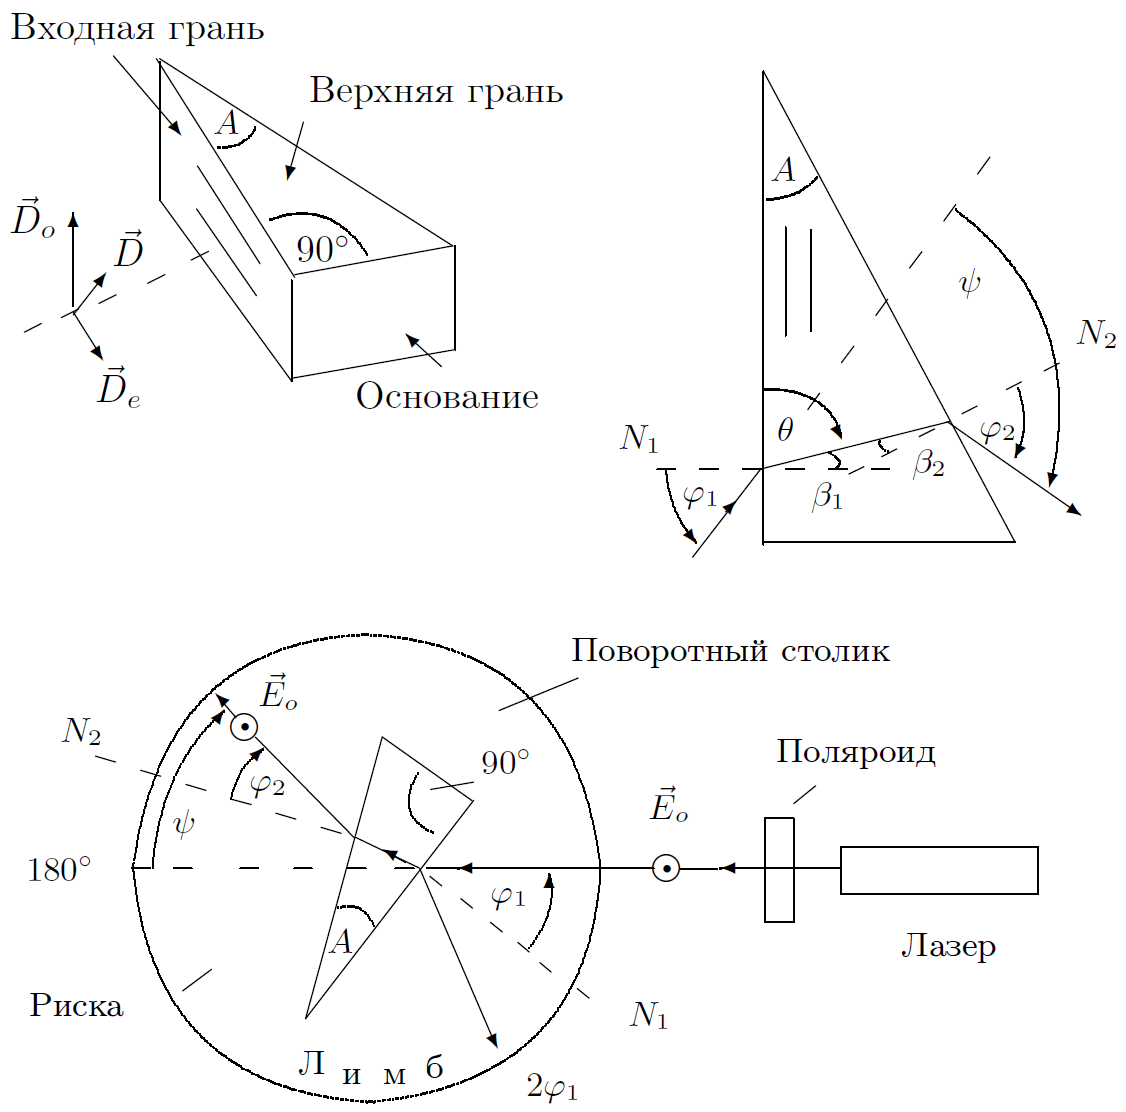
\includegraphics[scale = 0.7]{2.png}
	\end{center}
\end{figure}
 \newpage
 В работе использовался исландский шпат: $n_o = 1.655, n_e = 1.485$. Пользуясь приближением ${n_o} - {n_e} = 0.17 \ll {n_o},{n_e}$, упростим формулу для показателя преломления:
 \[n(\theta ) = {n_e} + ({n_o} - {n_e}){\cos ^2}\theta \]
 В результате получается график: 
 \begin{figure}[h!]
 	\begin{center}
 		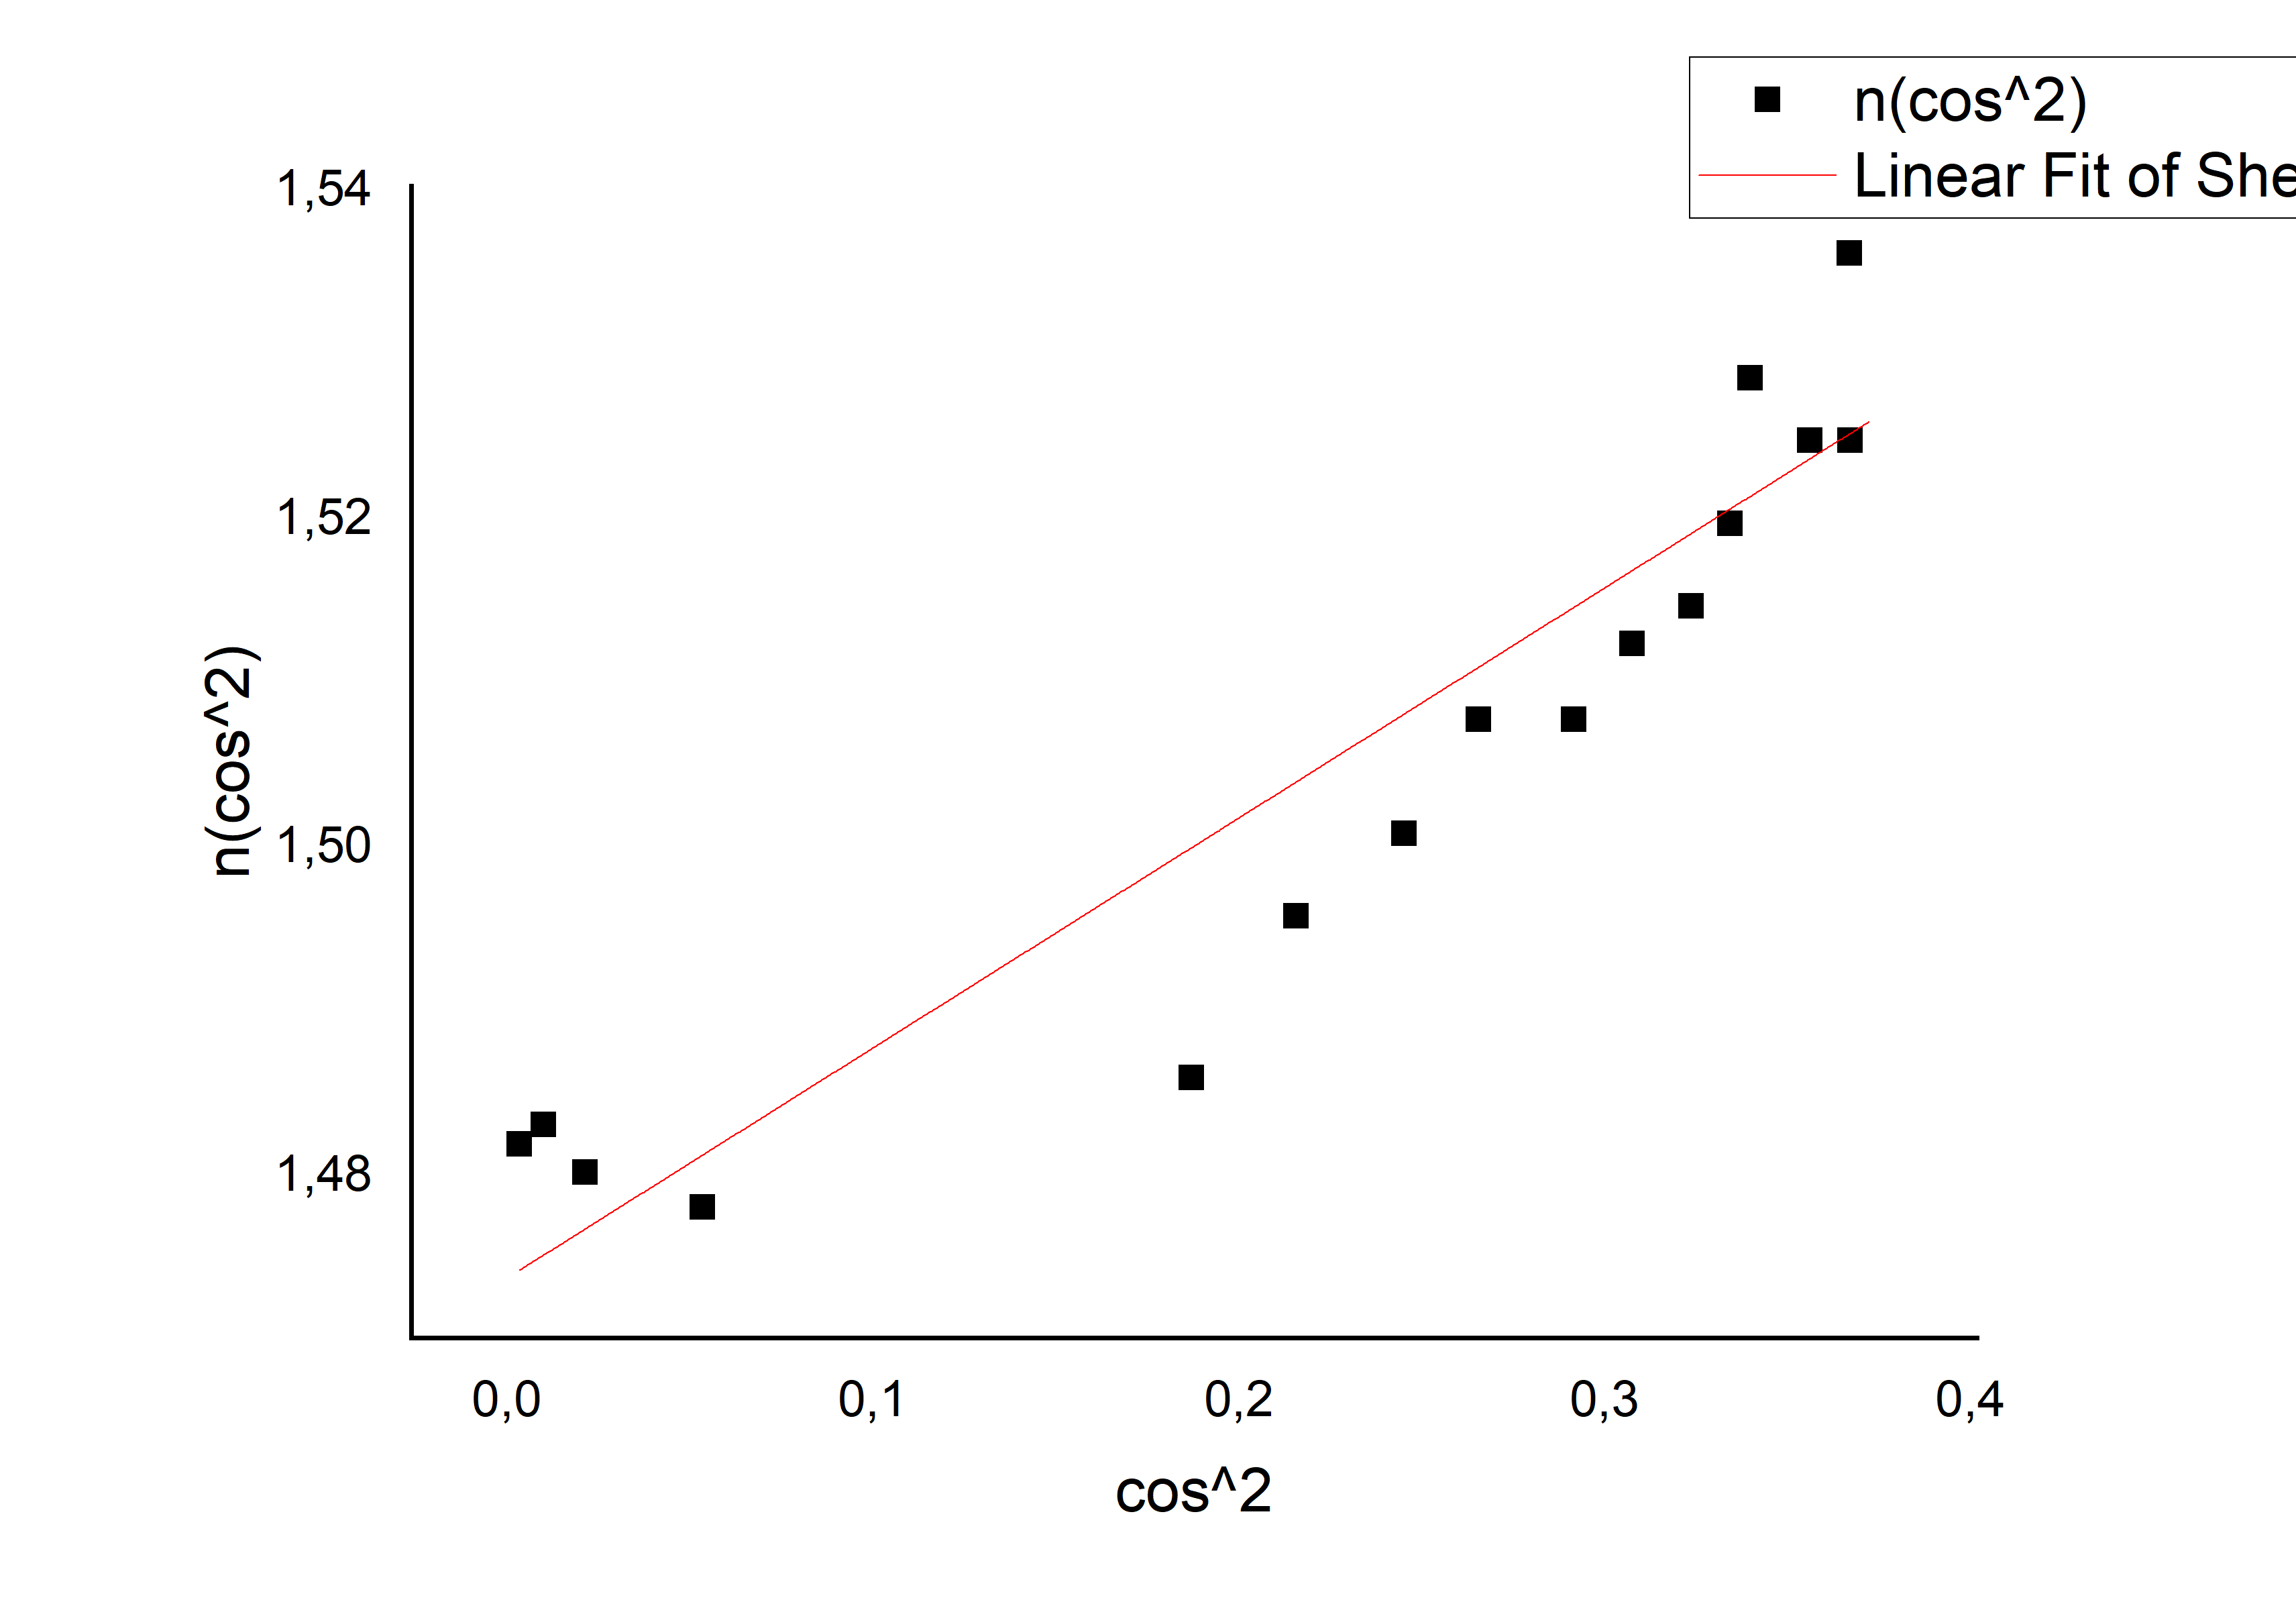
\includegraphics[scale = 0.4]{3.png}
 	\end{center}
 \end{figure}

Точка пересечения равна $1.47 \pm 0.02 \approx n_e$, наклон равен $0.15 \pm 0.03 \approx n_o-n_e$, что хорошо совпадает со справочными данными.

Зависомость также похожа на линейную, что согласуется с теорией.  
\end{document} % конец документа